\documentclass[titlepage,landscape]{seminar}
\usepackage{url}
\usepackage{graphicx}
\usepackage{hyperref}
\usepackage{epstopdf}
\usepackage{slides}

\newcommand{\frack}{\frac{1}{k}}
\newcommand{\quarter}{\frac{1}{4}}

\begin{document}

\myslide{
\heading{Ancestral polymorphism}

\begin{center}
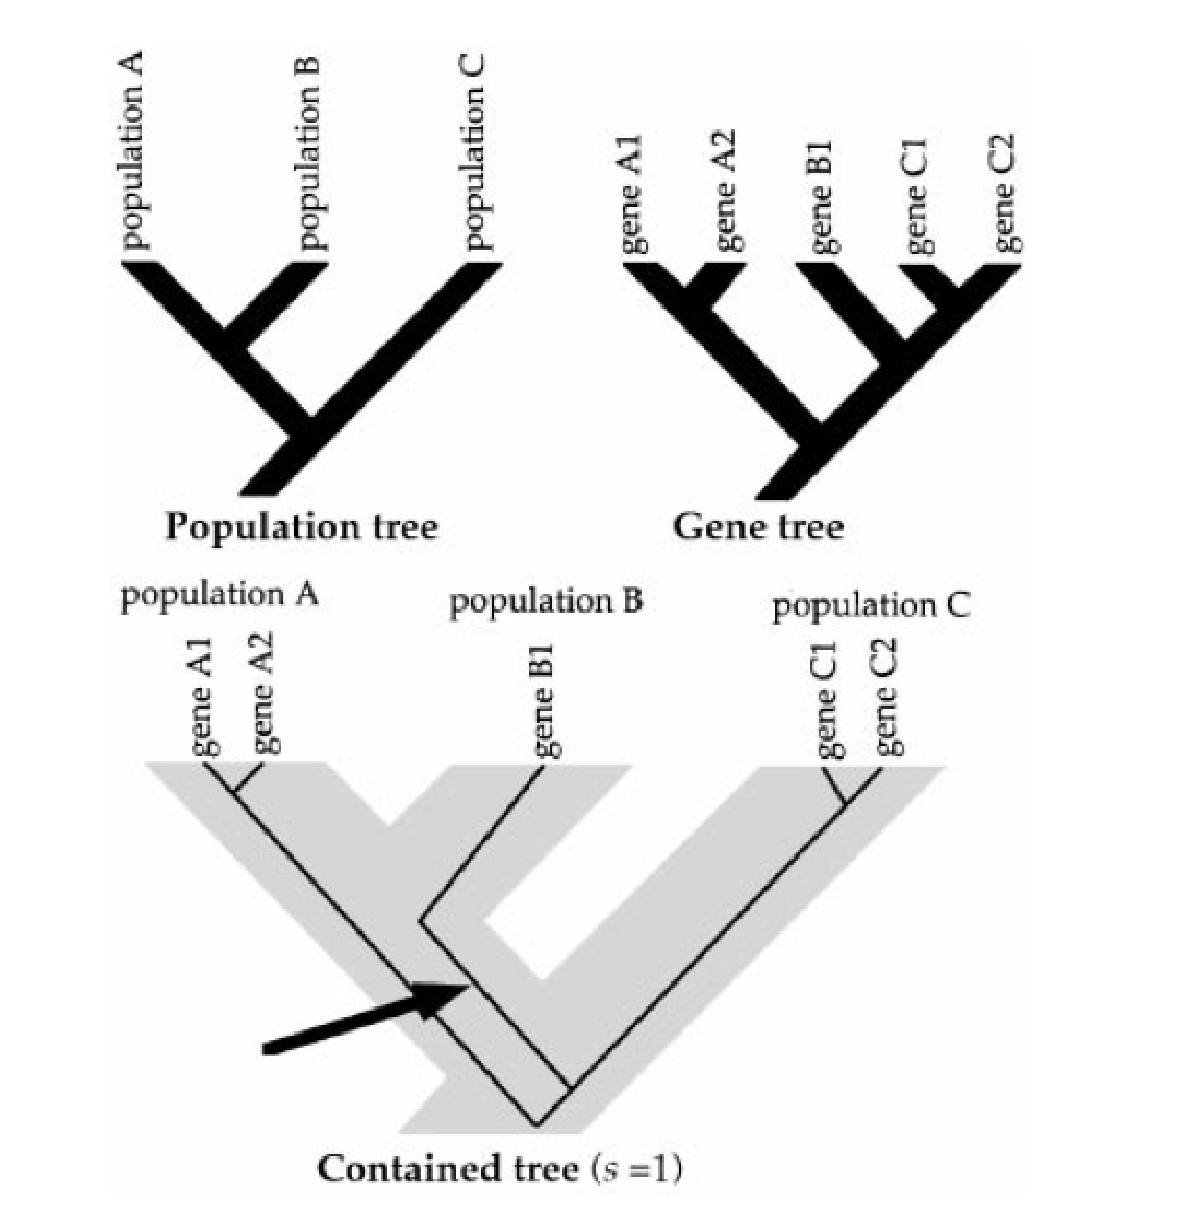
\includegraphics[height=0.9\textheight]{ancestral-polymorphism.eps}
\end{center}

}

\myslide{
\heading{The coalescent in structured populations}

Remember that in a single population
\[
P(t|k, N_e) = \left(\frac{k(k-1)}{4N_e}\right)\left(1-
  \frac{k(k-1)}{4N_e}\right)^{t-1}
\]

\begin{eqnarray*}
P_k(\mbox{coalescent}|n, N_e) &=& \frac{k(k-1)}{4N_e} \\
P(\mbox{no coalescent}|k, N_e, K)
                              &=&\left(1-\frac{k(k-1)}{4N_e}\right)^K \\
P(\mbox{no migration}|k,m, K) &=& (1-m)^{kK}
\end{eqnarray*}
}

\myslide{
\heading{The coalescent in structured populations}


{\scriptsize
\begin{eqnarray*}
P(\mbox{event}|k, m, N_e, K) &=& 1 - P(\mbox{no coalescent}|k, N_e,
K)P(\mbox{no migration}|k,m, K)
\end{eqnarray*}
}

{\small
\[
P(\mbox{event at }t|k, m, N_e, K) = P(\mbox{event}|k, m, N_e,
K)\left(1 - P(\mbox{event}|k, m, N_e, K)\right)^{t-1} 
\]

\[
P(\mbox{data}|m, N_e) \propto f(n, m, N_e, K)
\]

}
\vfill
\noindent Implemented in {\tt Migrate-N} developed by Peter Beerli

}

\myslide{
\heading{{\tt Migrate-N}: Limitations}

\begin{itemize}

\item {\bf Very} difficult to estimate more than a few migration
  parameters, even if there are multiple populations in the sample. 

\item Estimates of $\theta$ depend on model of mutation.

\item Underlying assumption that recent common ancestry among
  populations reflects {\it only\/} migration. Neglects possibility
  that recent common ancestry could reflect recent separation of
  populations. 

\end{itemize}
}

\myslide{
\heading{Population divergence and migration}
Basic model involves two populations that diverged an unknown number
of generations ago and that exchange migrants.

\begin{itemize}

\item $\theta_a$: $4N_e\mu$ in the ancestral population.

\item $\theta_1$: $4N_e\mu$ in the first population.

\item $\theta_2$: $4N_e\mu$ in the second population.

\item $M_1$: $2N_em_1$ in the first population, where $m_1$ is
  the fraction of the first population composed of migrants from the
  second population.

\item $M_2$: $2N_em_2$ in the second population.

\item $T$: time since the populations diverged. Specifically, if there
  have been $t$ units since the two populations diverged, $T=t/2N_1$,
  where $N_1$ is the effective size of the first population.

\end{itemize}
}

\myslide{
\heading{Population divergence and migration}
\begin{center}
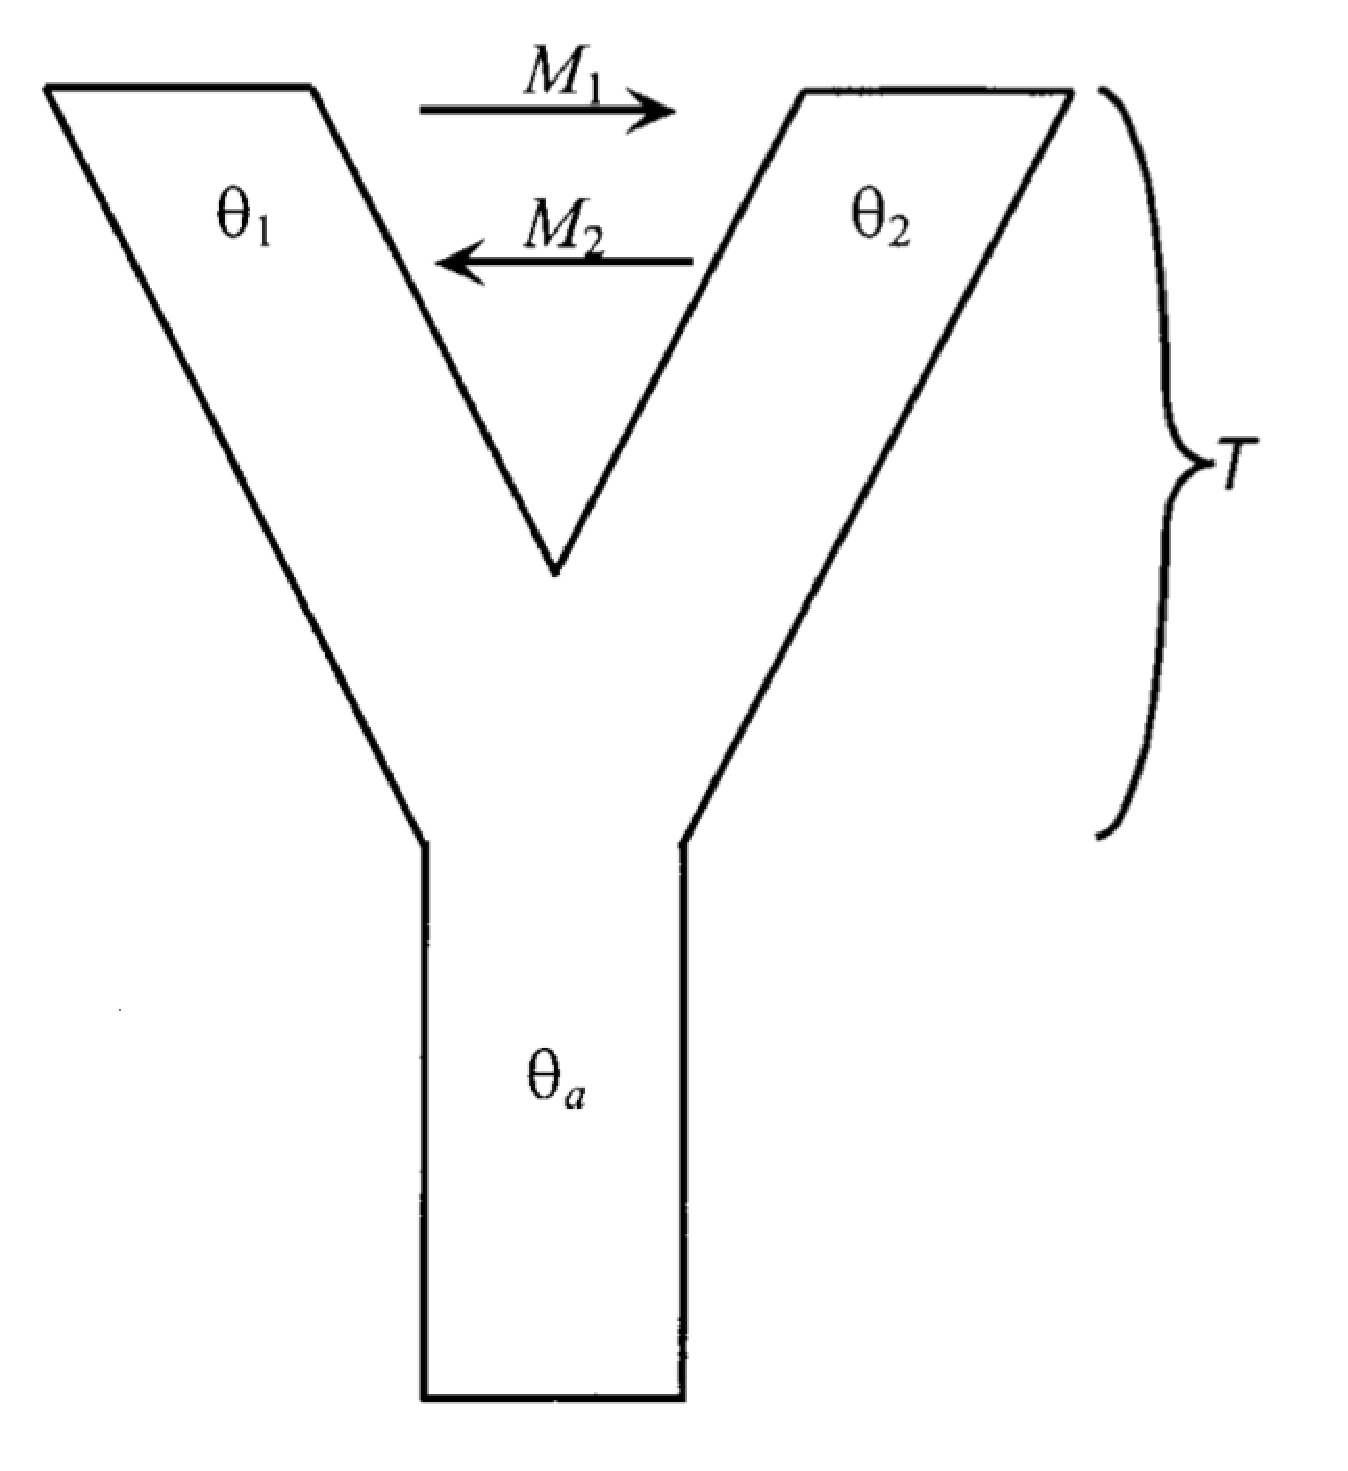
\includegraphics[height=0.9\textheight]{nielsen-wakeley.eps}
\end{center}
}

\myslide{
\heading{Population divergence and migration}

\begin{center}
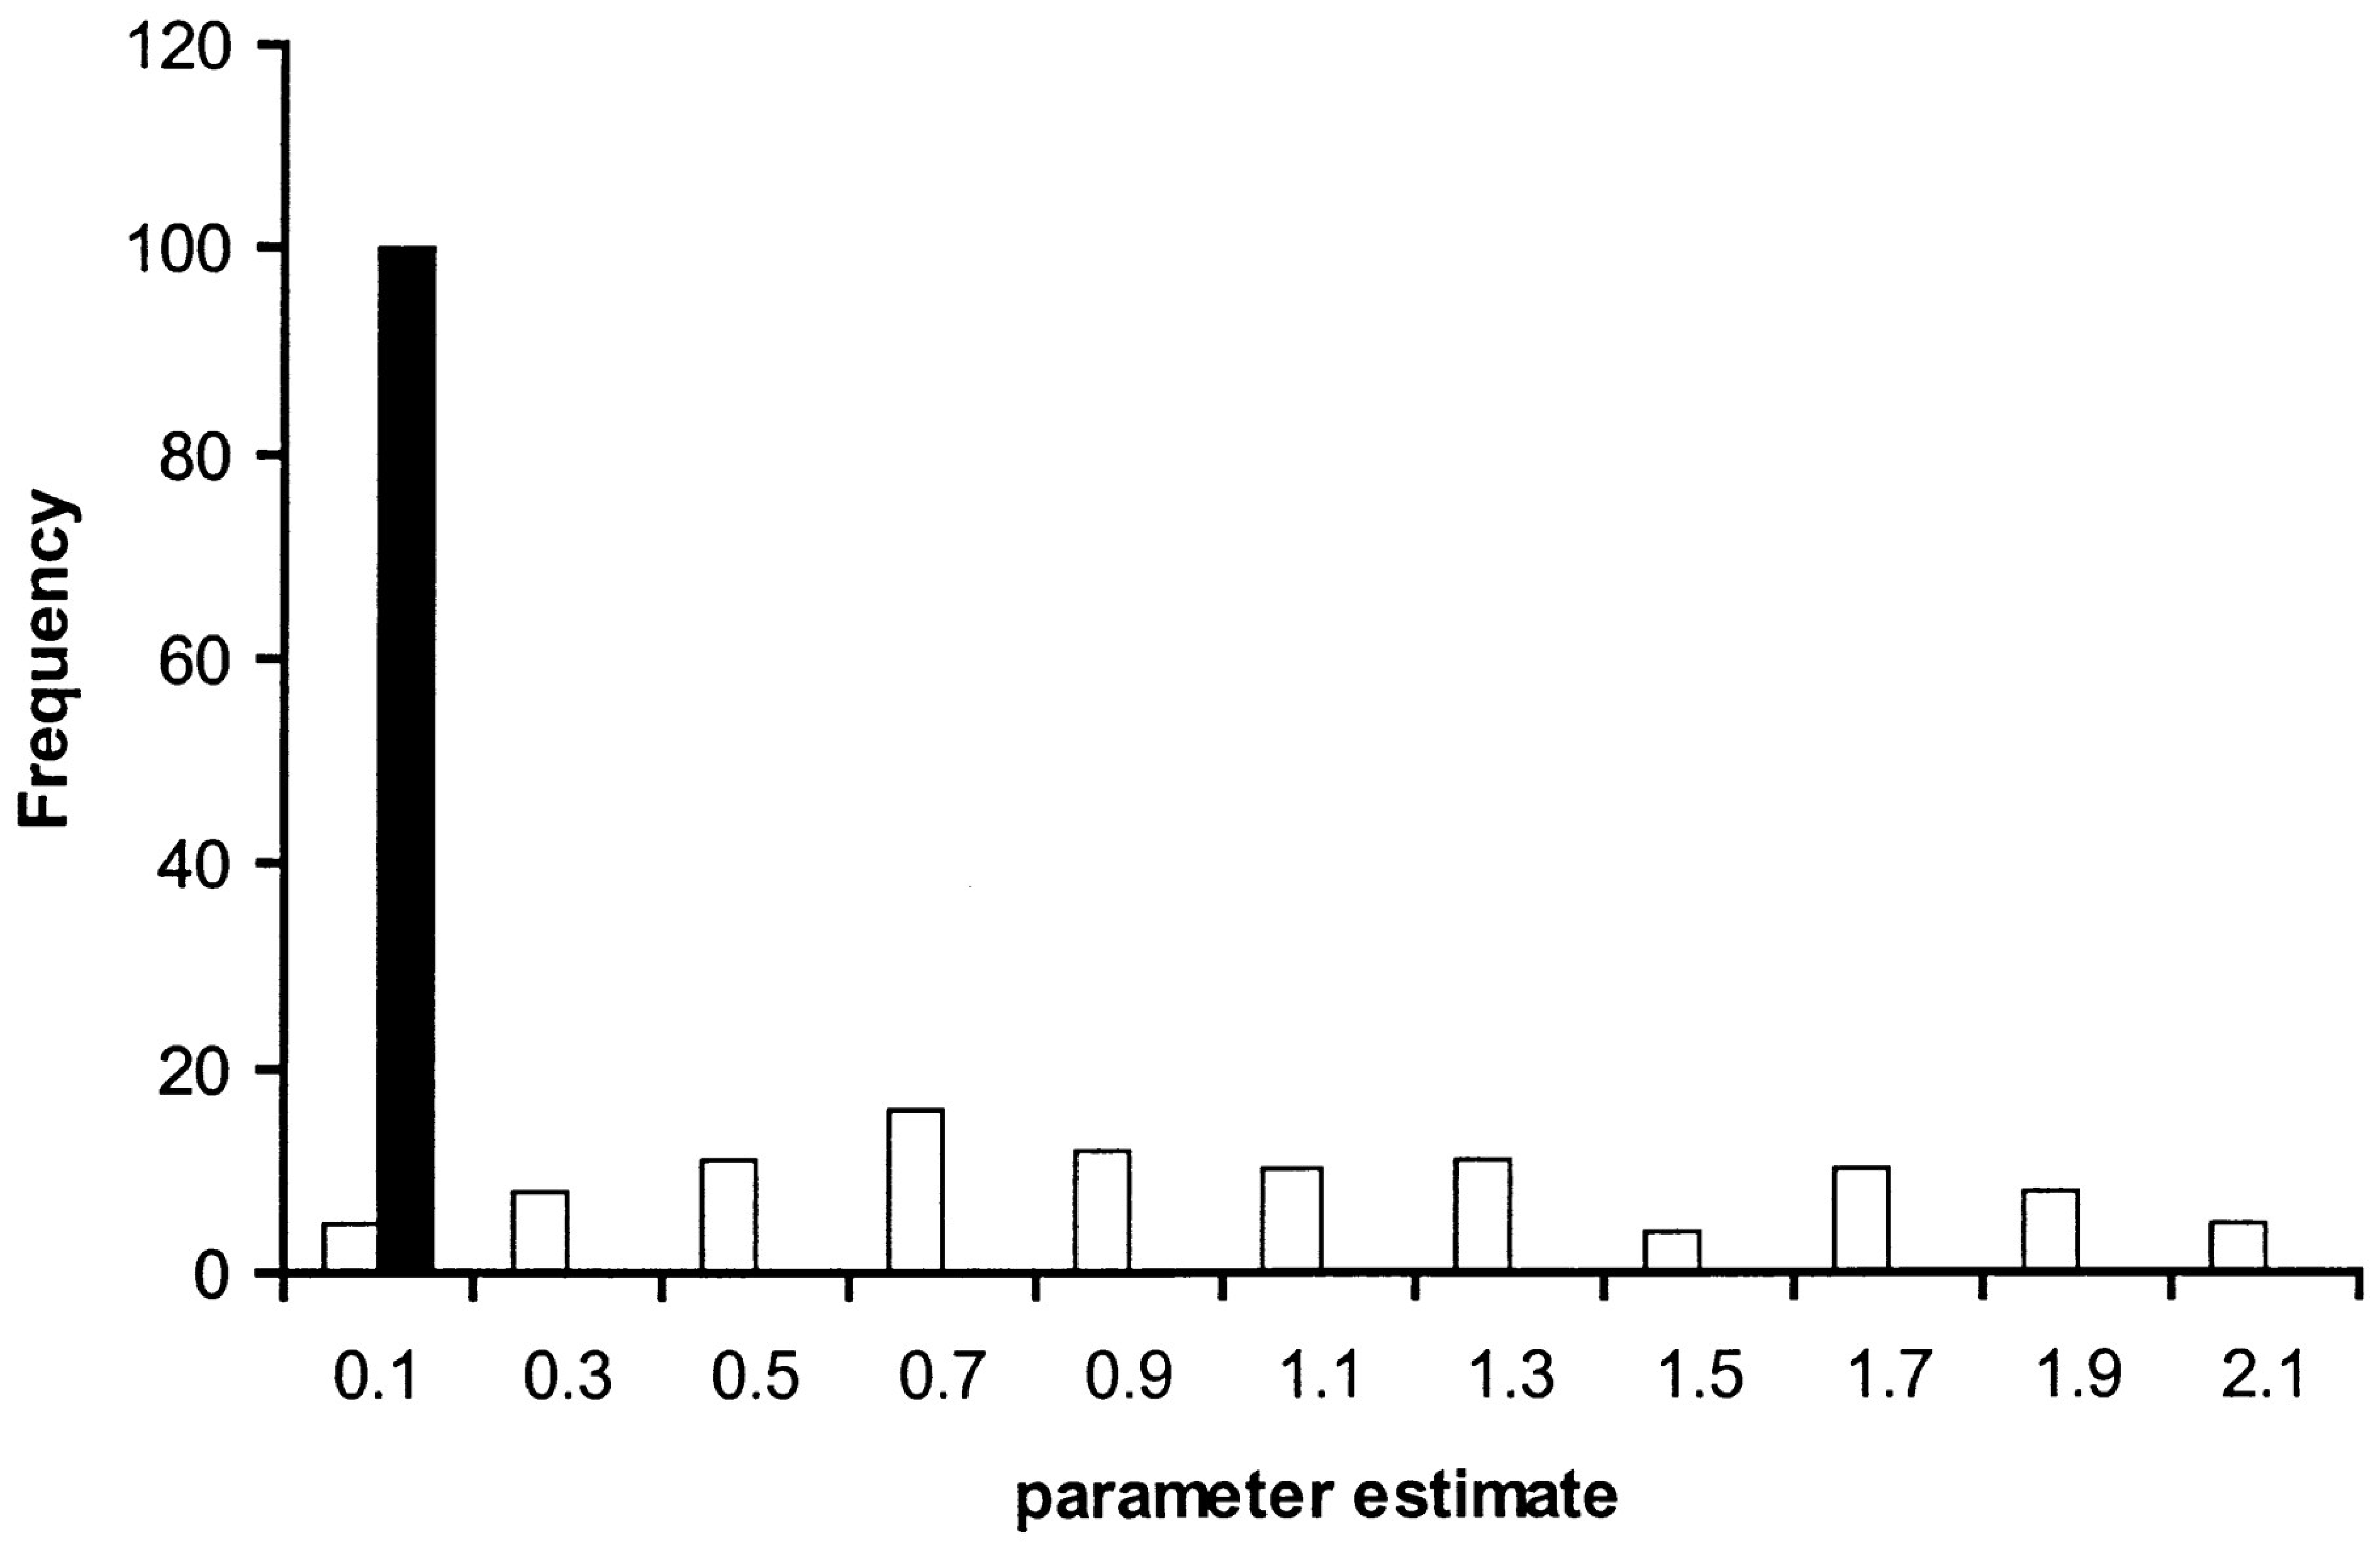
\includegraphics[height=0.7\textheight]{nielsen-wakeley-estimates.eps}
\end{center}
\vfil
{
\small
\noindent Open bars: $M_1 = 1.0$

\noindent Closed bar: $M_2 = 0.0$
}
}

\myslide{
\heading{Population divergence and migration: example}

Orti et al.~(1994) mtDNA sequences from 25 populations of threespine
stickleback, {\it Gasterosteus aculeatus}

\begin{itemize}

\item Europe, North America, Japan

\item 747bp fragment of cytochrome $b$

\end{itemize}
}

\myslide{
\heading{Population divergence and migration}

\begin{center}
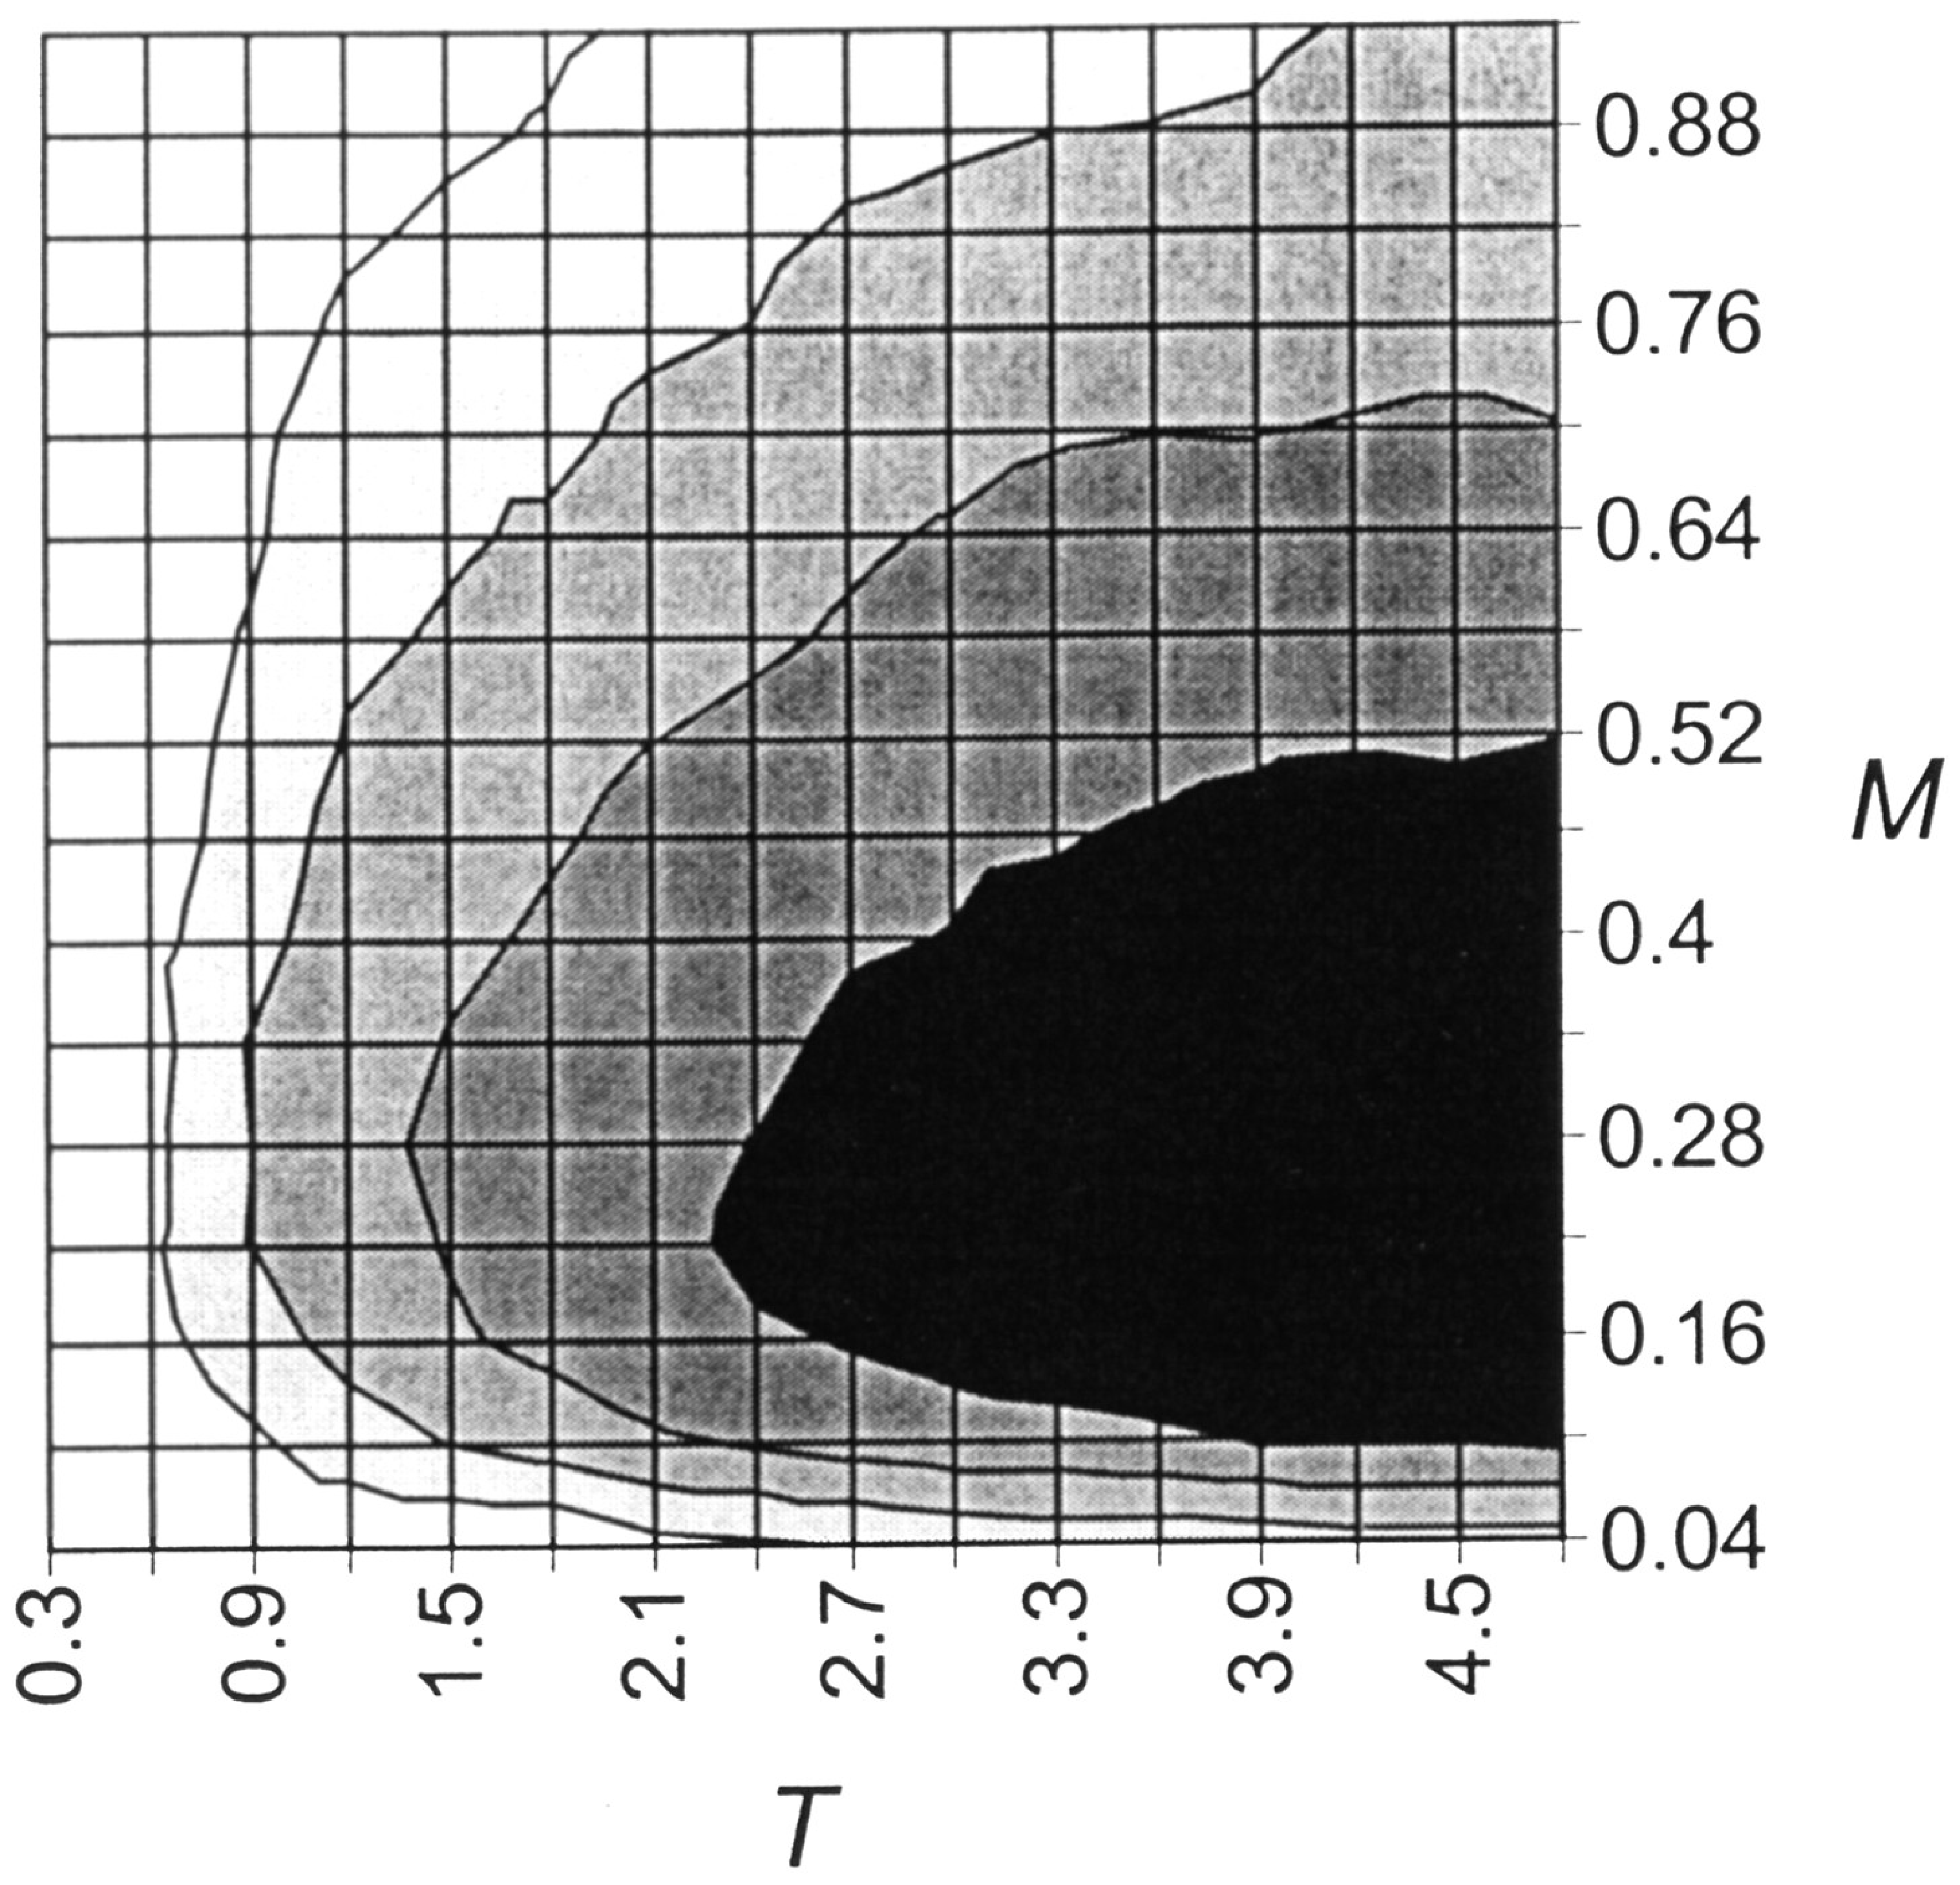
\includegraphics[height=0.9\textheight]{nielsen-wakeley-tm.eps}
\end{center}

}

\myslide{
\heading{Population divergence and migration}

\begin{center}
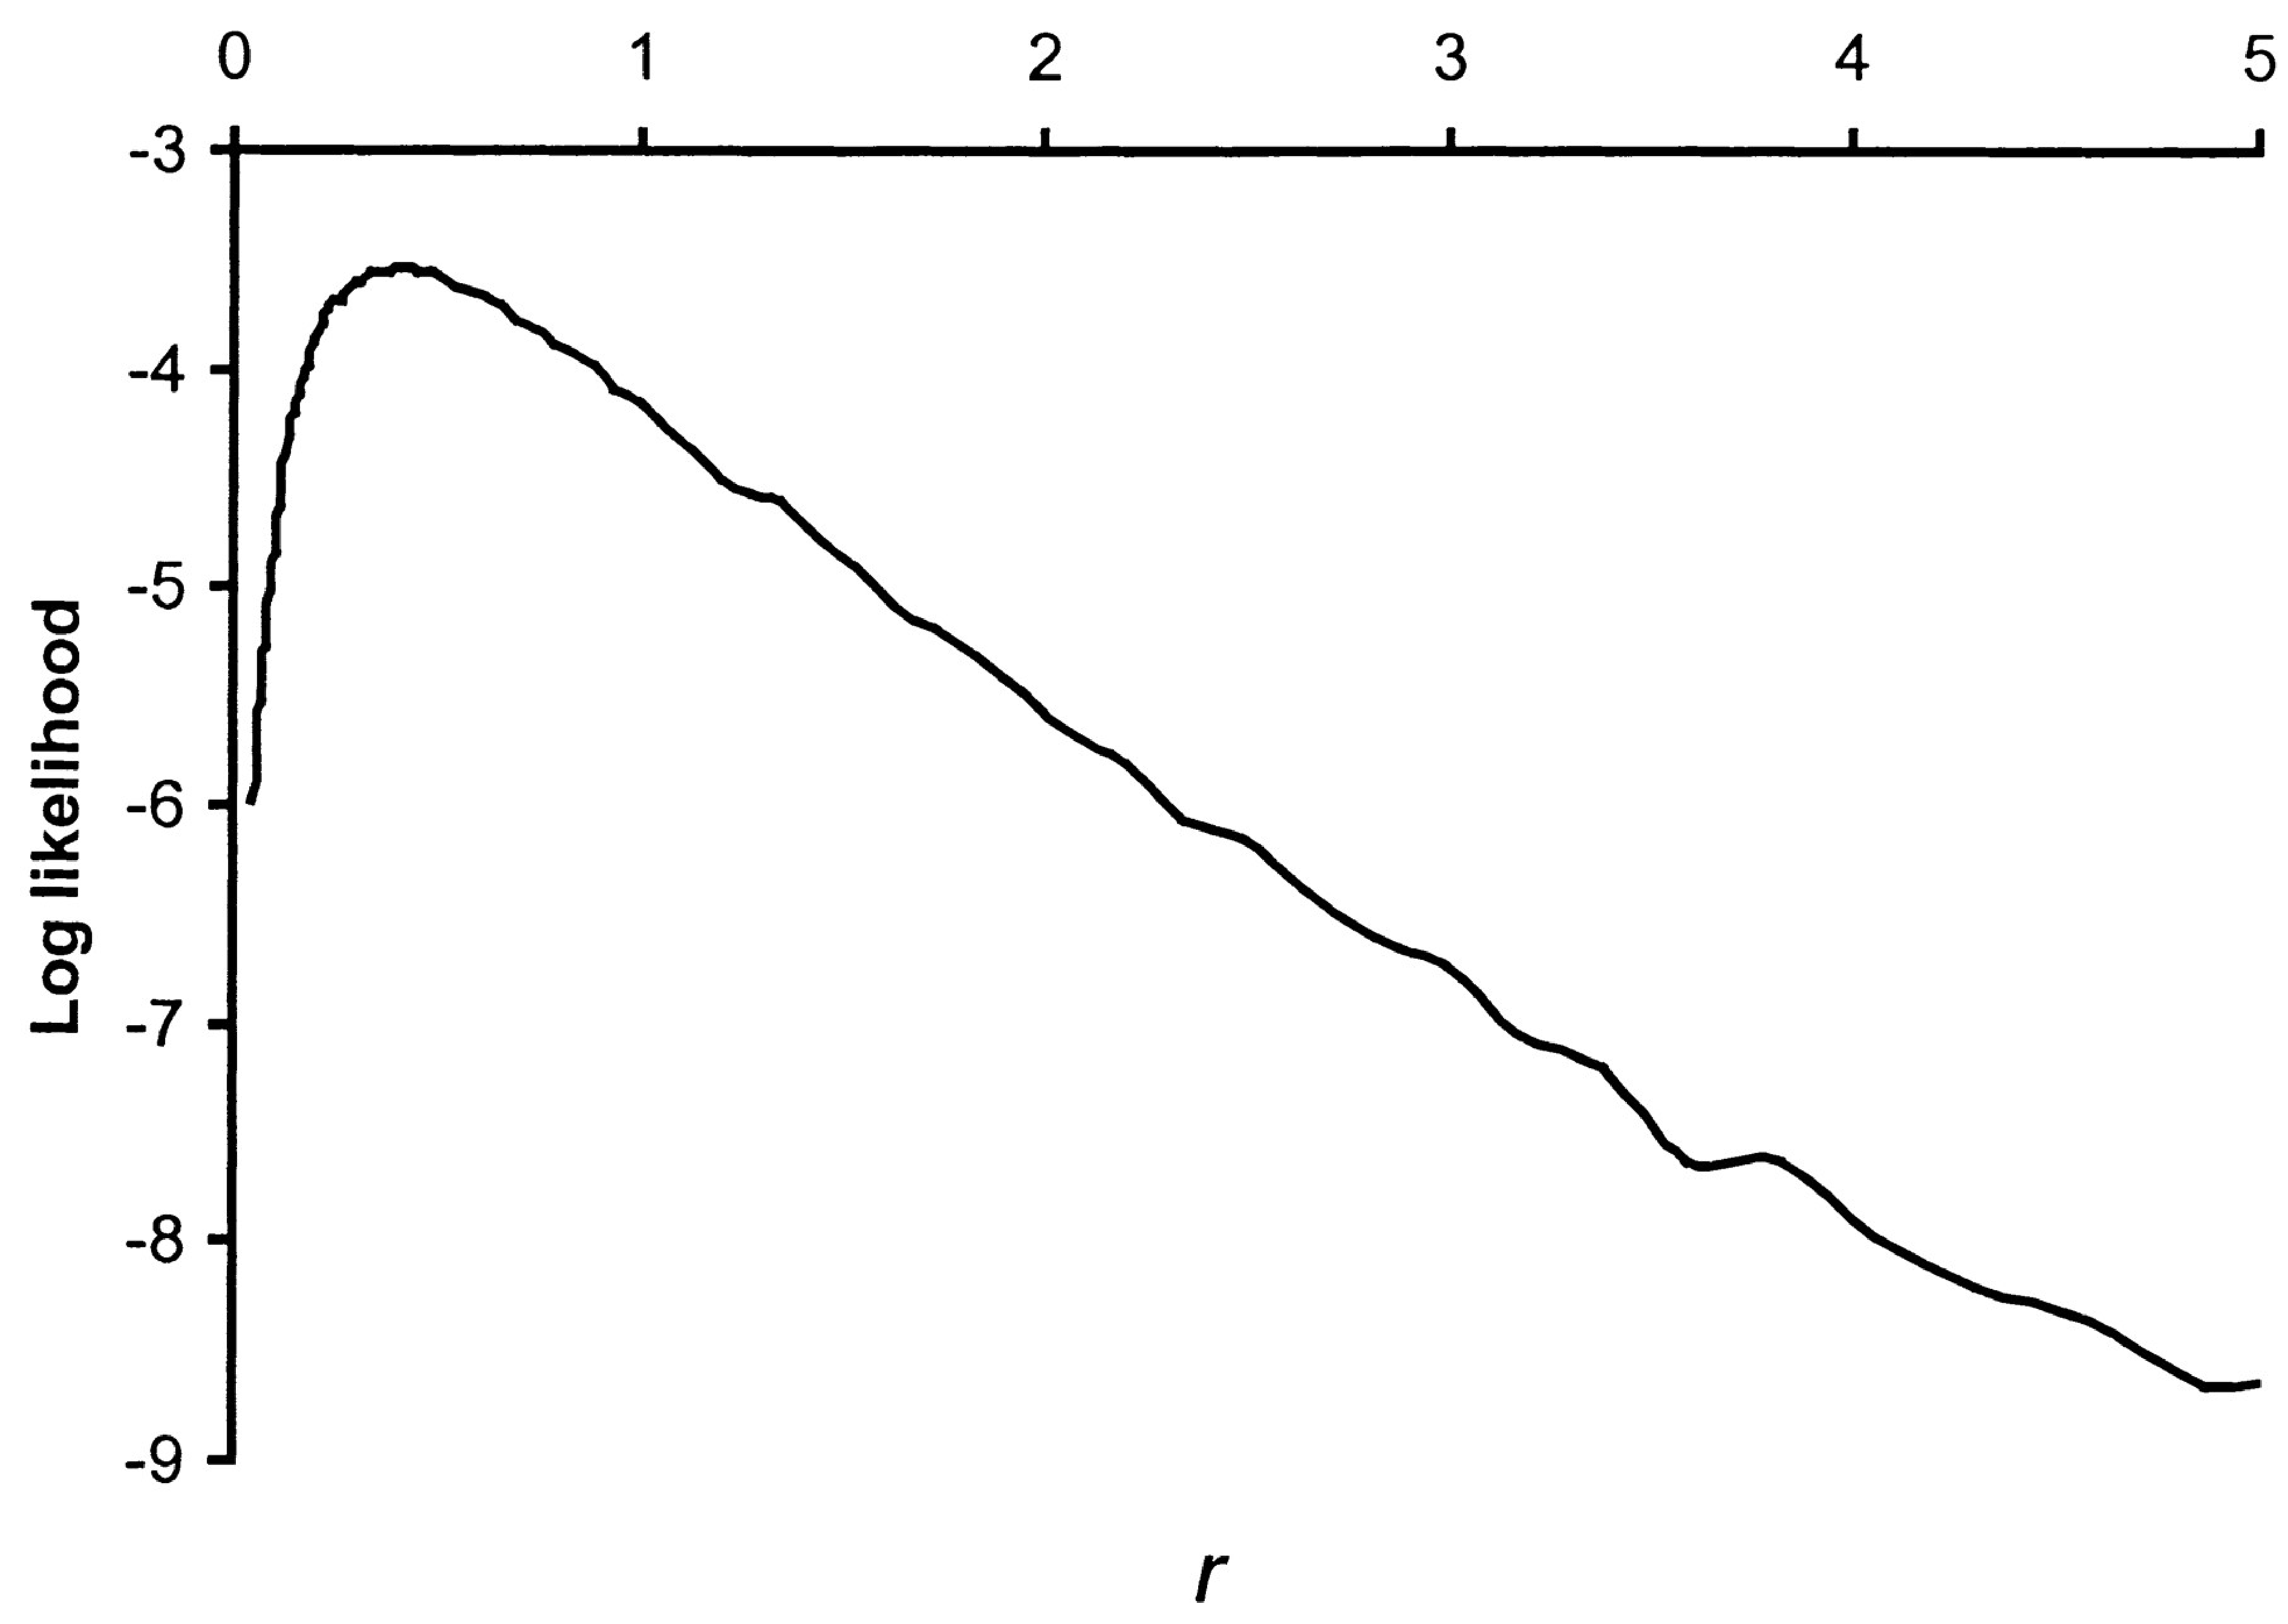
\includegraphics[height=0.8\textheight]{nielsen-wakeley-thetas.eps}
\end{center}
\vfil
\[
r = \frac{N_2}{N_1}
\]

}

\myslide{
\heading{{\it Melanopus oregonensis}}
\begin{center}
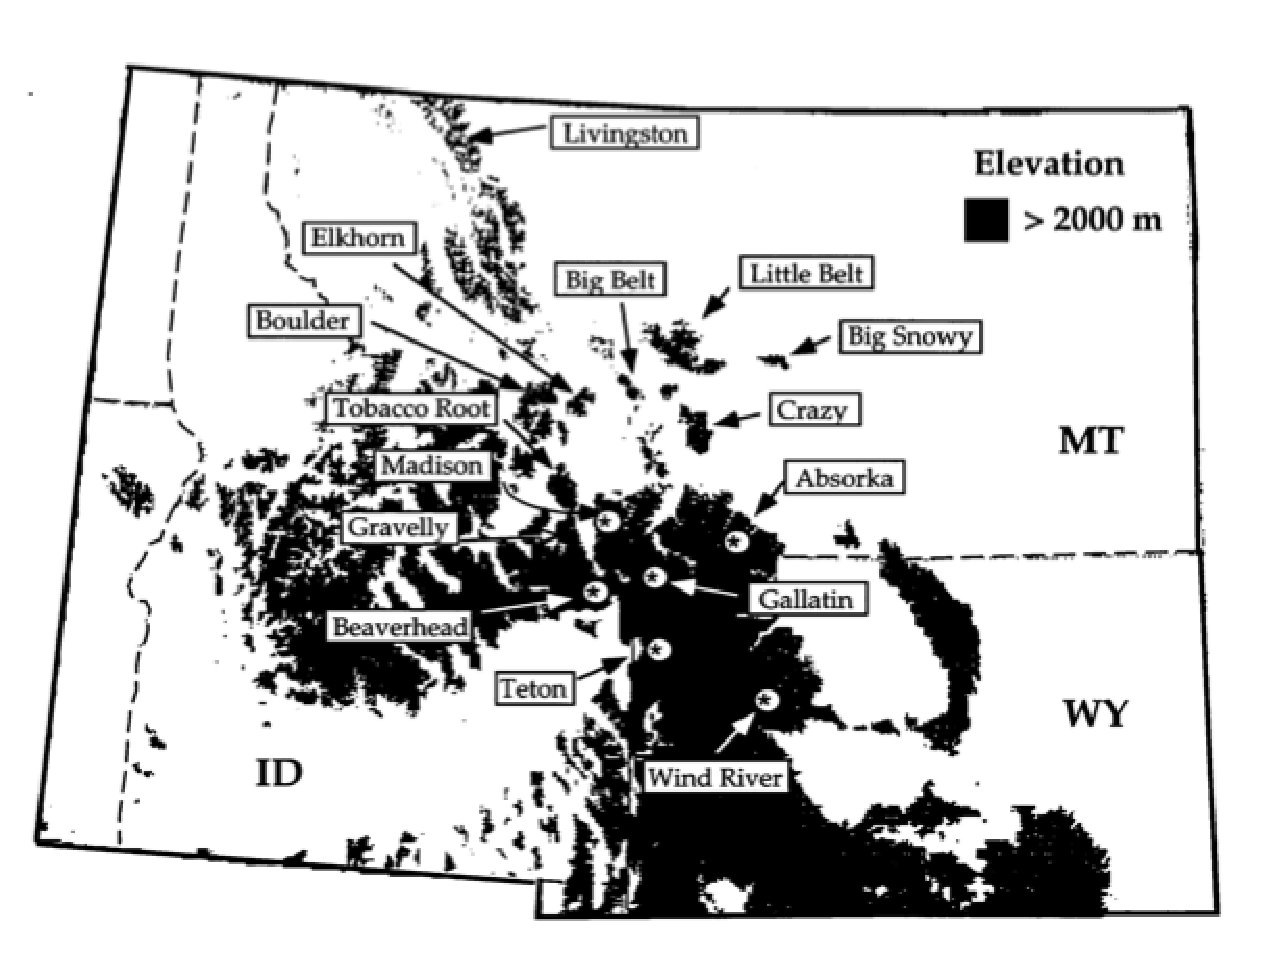
\includegraphics[height=0.9\textheight]{sky-islands.eps}
\end{center}
}

\myslide{
\heading{{\it Melanopus oregonensis}}
\begin{itemize}

\item {\bf Widespread ancestor}: The existing populations might represent
  independently derived remnants of a single, widespread
  population. In this case all of the populations would be equally
  related to one another.

\item {\bf Multiple glacial refugia}: Populations that shared the same
  refugium will be closely related while those that were in different
  refugia will be distantly related.

\end{itemize}
}

\myslide{
\heading{{\it Melanopus oregonensis}}
\begin{center}
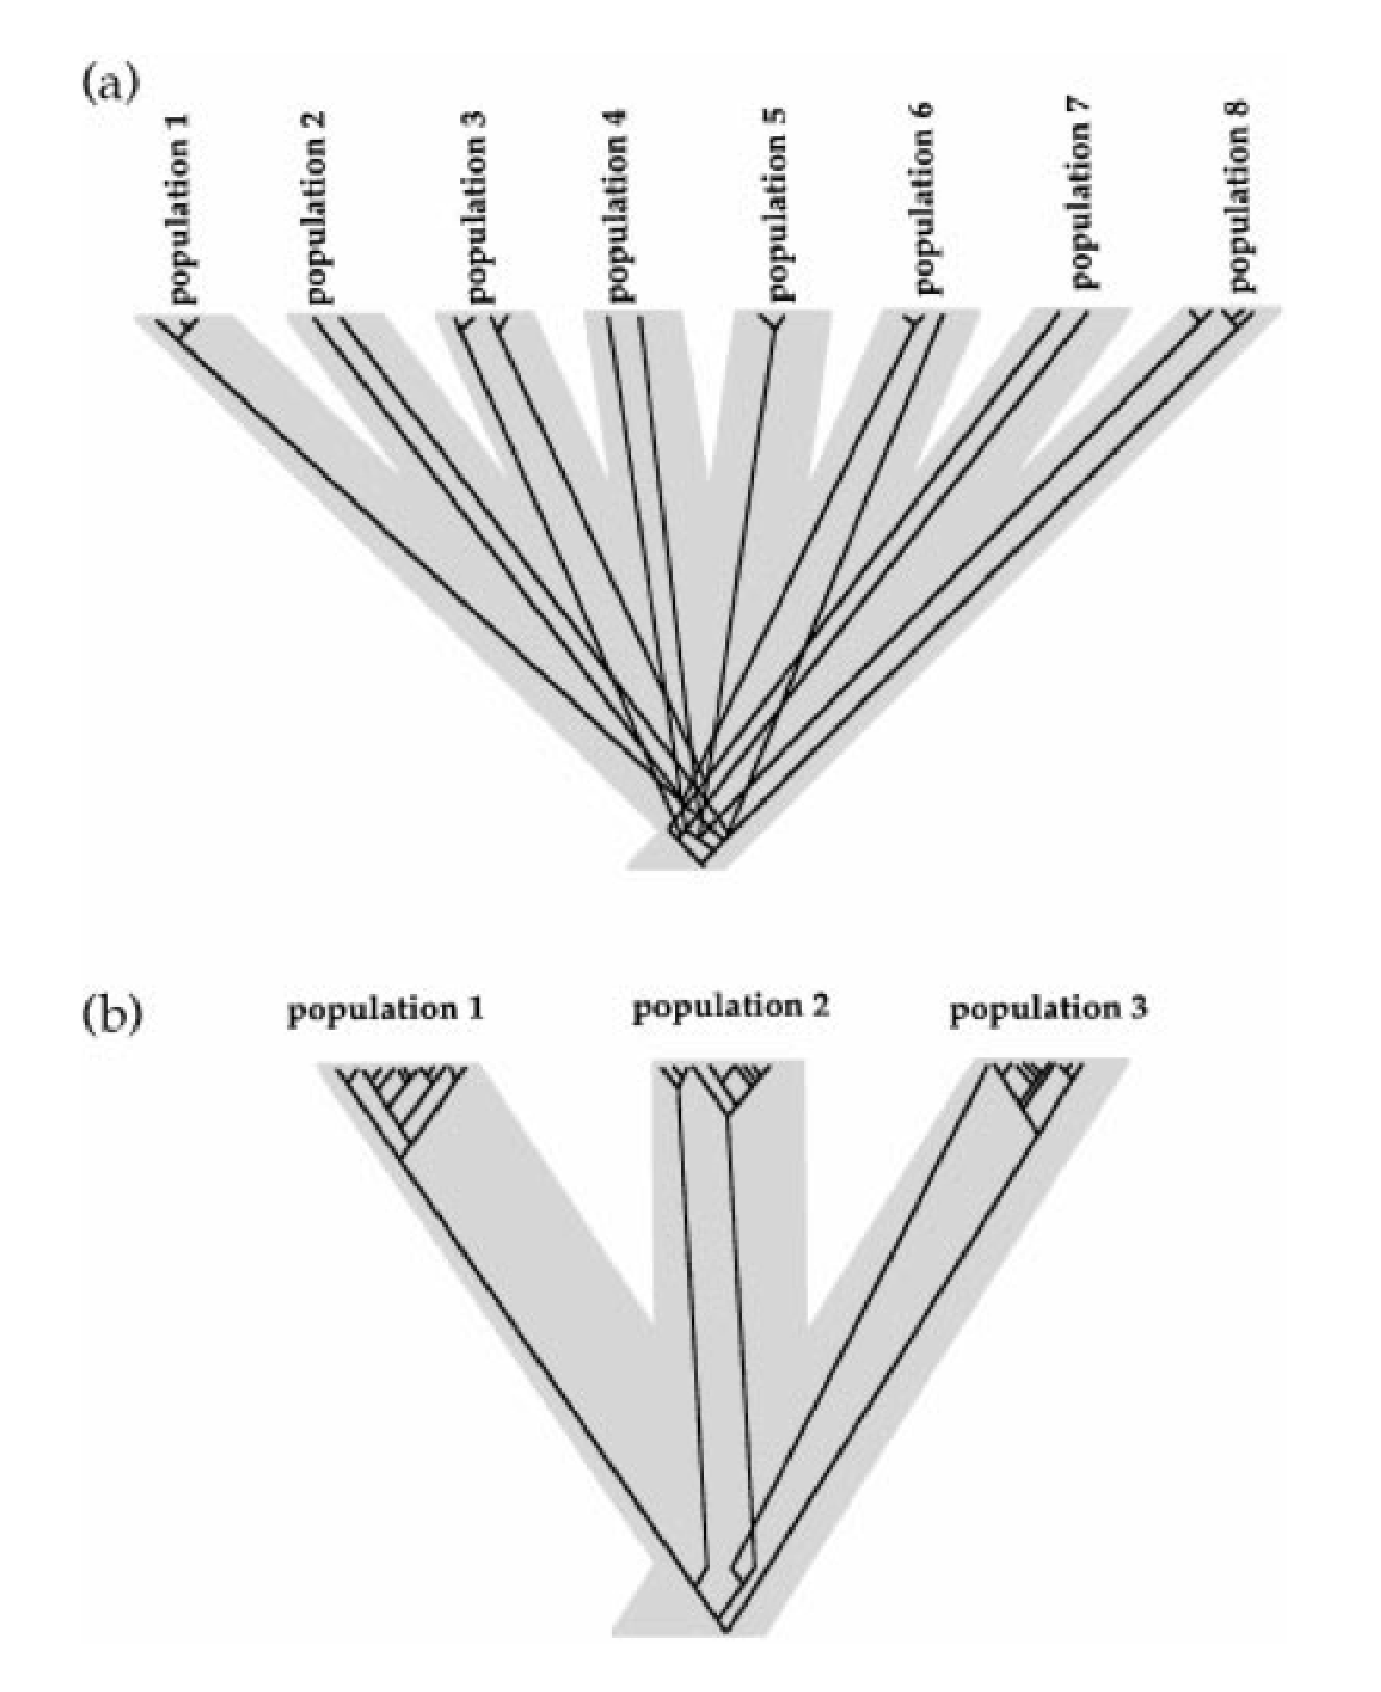
\includegraphics[height=6cm]{divergence-hypotheses.eps}
\end{center}
}

\myslide{
\heading{{\it Melanopus oregonensis}}
\begin{itemize}

\item Estimate the the phylogeny of the haplotypes in the sample. 

\item Estimate $s_{obs}$,  the minimum number of among-population  migration
  events necessary to account for where haplotypes are currently found
  given the inferred phylogeny.

\item Simulate a neutral coalescence process in which the populations
  are derived from a single, widespread ancestral population. 

\item Rearrange the data so that populations are grouped into separate
  refugia.

\item Estimate $s_{sim}$ from the rearranged data, and repeat this 100
  times for several different times since population splitting.

\end{itemize}
}

\myslide{
\heading{{\it Melanopus oregonensis}}
\begin{center}
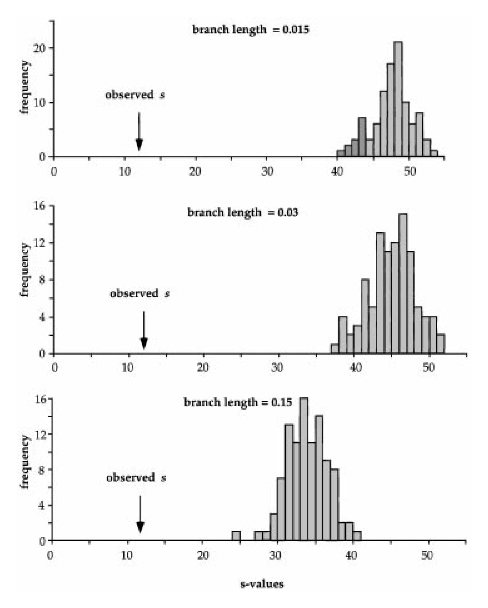
\includegraphics[height=0.9\textheight]{knowles-s-values.eps}
\end{center}
}

\myslide{
\heading{{\it Bufo marinus}}
\begin{center}
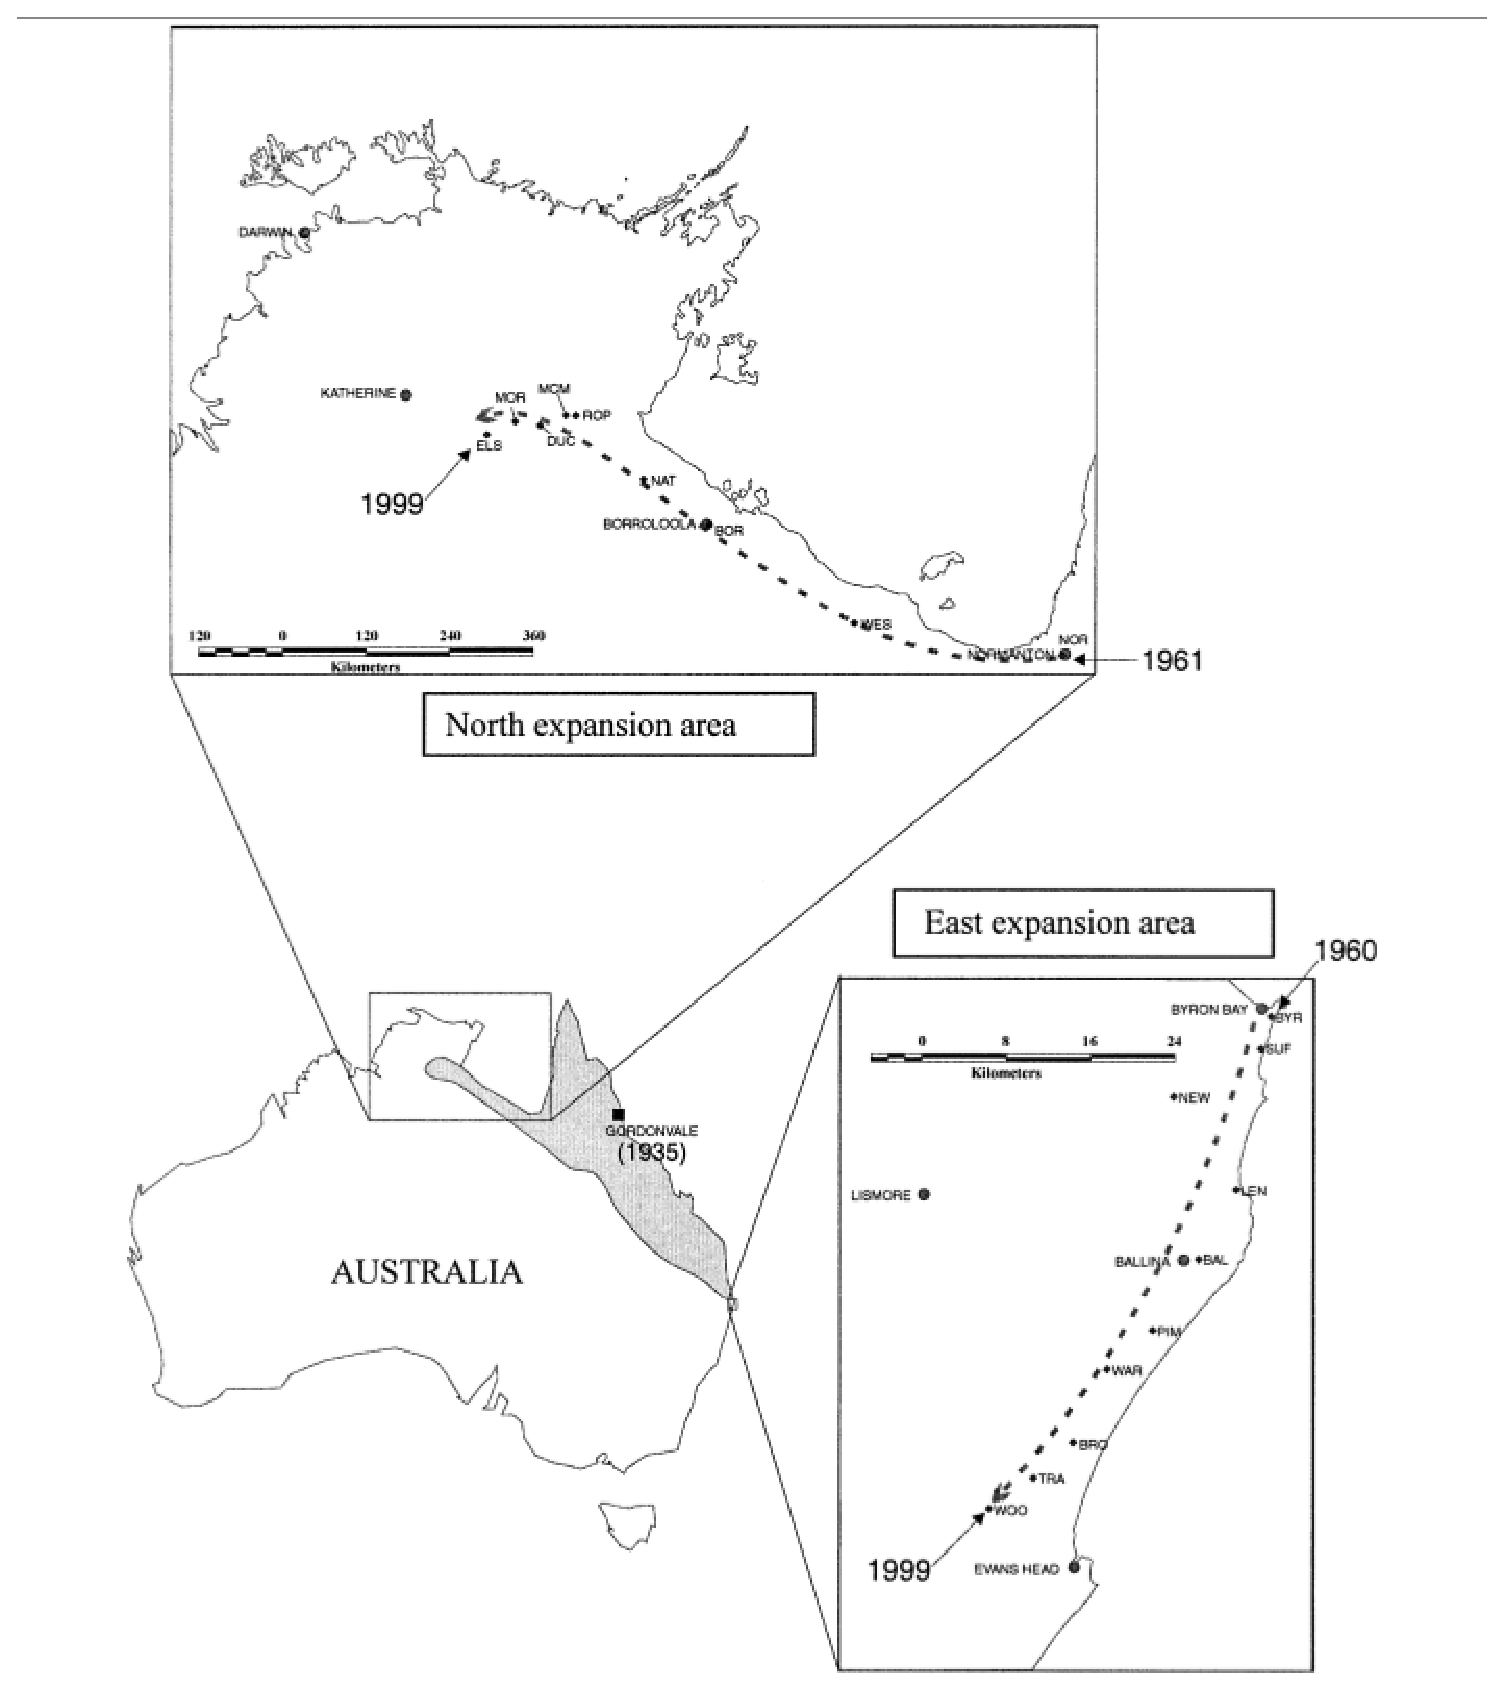
\includegraphics[width=0.8\textheight]{cane-toad-expansion.eps}
\end{center}
}

\myslide{
\heading{{\it Bufo marinus}}
\begin{enumerate}

\item Isolation by distance

\item Differential migration and founding

\item ``Island'' migration and founding

\item Stepwise migration and founding with founder events

\item Stepwise migration and founding without founder events

\end{enumerate}
}

\myslide{
\heading{Approximate Bayesian Computation (ABC)}
\[
\mbox{P}(X|\xi) = \mbox{likelihood of data, $X$, given parameters $\xi$}
\]
\vfill
\begin{enumerate}

\item Calculate ``appropriate'' summary statistics for your data set,
  $S$. 

\item Specify a prior distribution for the unknown parameters, $\xi$.

\item Pick $\xi'$ from the prior distribution and simulate data.

\item Calculate $S'$ from the simulated data.

\item Calculate the distance, $\delta$ between $S$ and $S'$.

\item If $\delta < \delta_{max}$, keep $S'$ and $\xi'$. Otherwise,
  discard them. 

\item Return to step 3 and repeat until you you have accepted a large
  number of pairs of $S'$ and $\xi'$.

\end{enumerate}
}

\myslide{
\heading{Approximate Bayesian Computation (ABC)}
\vfill
Fit the following regression:
\[
\xi_i = \alpha + S_i\beta + \epsilon 
\]
\vfill
``Predict'' $\xi$ for our observed data
\[
\xi = \alpha + S\beta + \epsilon 
\]
}

\myslide{
\heading{{\it Bufo marinus}}
\begin{center}
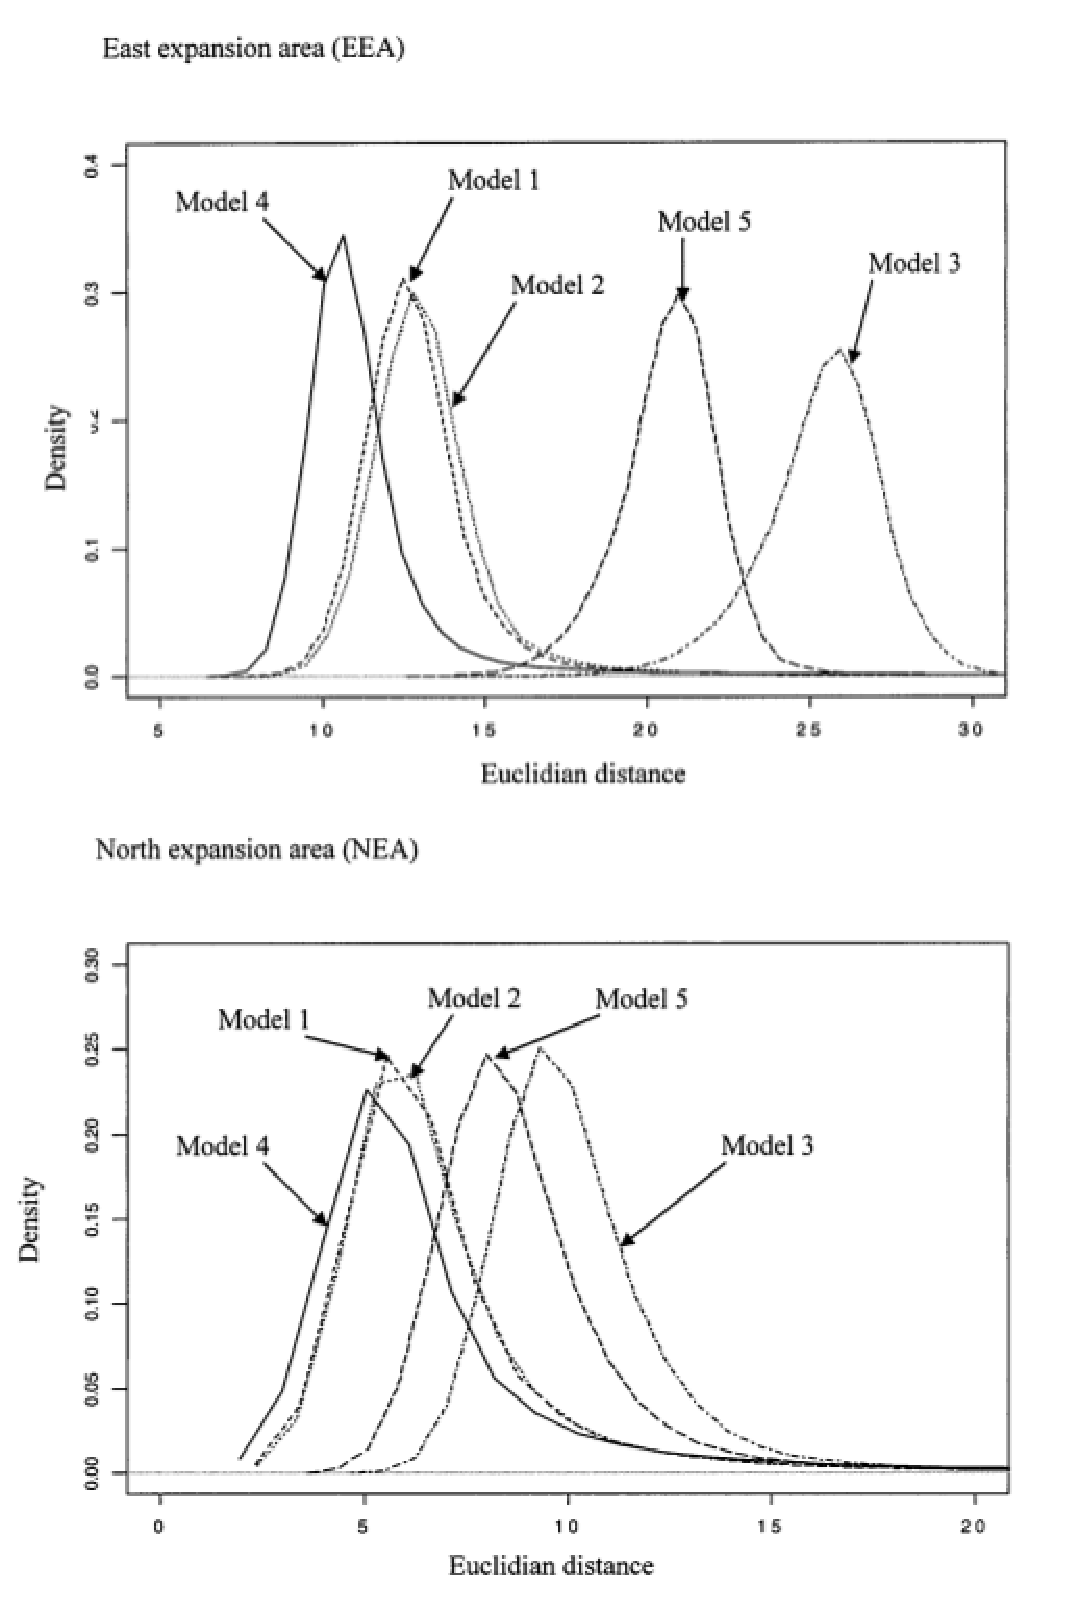
\includegraphics[height=0.9\textheight]{cane-toad-models.eps}
\end{center}
}

\myslide{
\heading{{\it Bufo marinus\/} (Model 4)}
\begin{center}
\begin{tabular}{ccr}
\hline\hline
Parameter & area & mean (5\%, 90\%) \\
\hline
$N_{e_s}$ & east & 744 (205, 1442) \\
         & north & 1685 (526, 2838) \\
$N_{e_f}$ & east & 78 (48, 118) \\
         & north & 311 (182, 448) \\
$F_R$    & east & 10.7 (2.4, 23.8) \\
         & north & 5.9 (1.6, 11.8) \\
$m$      & east & 0.014 ($6.0 \times 10^{-6}$, 0.064) \\
         & north & 0.117 ($1.4 \times 10^{-4}$, 0.664) \\
$N_{e_s}m$ & east & 4.7 (0.005, 19.9) \\
          & north & 188 (0.023, 883) \\
\hline
\end{tabular}
\end{center}
}
\end{document}


